\chapter{驱动程序的设计和实现}

\section{设备驱动概述}
	通常为了实现与应用程序的平台无关性,操作系统都会为应用程序提供一套标准的接口,VxWorks也不例外,这样就可以通过调整底层驱动或者是接近驱动那部分的操作系统中间层来提高应用层开发的效率,避免重复编码。在我们的通用操作系统(如Mac OS、Linux、Windows)当中,通常会将这套应用层的接口标准从操作系统中独立出来,专门以标准库的形式存在,这样可以屏蔽操作系统之间的差异,增强应用程序的平台无关性。
	
	VxWorks中也对应用层提供了一套标准的文件操作接口,实际上与GPOS提供接口类似,我们将其称作为标准I/O 库,VxWorks下由ioLib.c文件提供。ioLib.c文件提供如下标准接口函数:creat()、open()、unlink()、remove()、close()、rename()、read()、write()、ioctl()、lseek()、readv()、writev()等\cite{BSP开发人员指南},VxWorks与通用操作系统有很大的一个不同点是:VxWorks不区分用户态和内核态,用户层可以直接对内核函数进行调用,而无需使用陷阱指令之类的机制,以及存在使用权限上的限制。因此VxWorks提供给应用层的接口无需通过外围库的方式,而是直接以内核文件的形式提供。
	
	设备驱动时直接控制设备操作的那部分程序,也是设备上层的一个软件接口。设备驱动程序的功能完成软件层对硬件的访问,实际上从软件工程的角度来说就是介于软件和硬件之间实现软件层标准接口的程序。软件层访问硬件必须要通过调用驱动程序。所以驱动程序不能自动执行,只能被系统或者程序调用。
	
	应用程序必须要通过驱动程序才能够与硬件设备进行通信,而驱动程序的编写与操作系统的关系密不可分。设备驱动程序在操作系统中如何存在、如何与操作系统的其它部分相联系、如何与操作系统的其他部分相联系、如何为用户提供服务都是操作系统的设计人员在设计操作系统时制定的,系统已经为驱动程序制定好了一个框架,无论驱动程序的开发人员以何种方式控制设备,他们所开发的驱动程序都是以预先设计好的方式存在、与操作系统其他部分相联系和为用户提供服务的。将这种由操作系统的设计人员指定的设备驱动程序结构定义为驱动程序的外部结构,而由于驱动开发人员在开发设备驱动时采用的具体策略不同导致的不同的驱动程序结构称为驱动程序的内部结构。驱动程序的外部结构决定了操作系统的I/O体系结构,驱动程序的内部结构决定了不同的设备驱动方式。

	在VxWorks系统中,在控制器权转到设备驱动程序之前,用户的请求进行尽可能少的处理。VxWorks I/O系统的角色更像是一个转接开关,负责将用户请求转接到合适的驱动例程上。每一个驱动都能够处理原始的用户请求,到最合适它的设备上。另外,驱动程序开发者也可以利用高级别的库例程来实现基于字符设备或者块设备的标准协议。因此,VxWorks的I/O系统具有两方面的优点:一方面使用尽可能少的使用驱动相关代码就可以为绝大多数设备写成标准的驱动程序,另一方面驱动程序开发者可以在合适的地方使用非标准的程序自主的处理用户请求。


\subsection{设备驱动的功能以及组成部分}
\subsubsection{设备驱动程序结构}
	VxWorks 的I/O框架由ioLib.c 文件提供,但ioLib.c文件提供的函数仅仅是一个最上层的接口,并不能完成具体的用户请求,而是将请求进一步向其他内核模块进行传递,位于ioLib.c模块之下的模块就是iosLib.c。我们将ioLib.c 文件称为上层接口子系统,将iosLib.c文件称为I/O 子系统,注意二者的区别。上层接口子系统直接对用户层可见,而I/O 子系统则一般不可见(当然用户也可以直接调用iosLib.c 中定义的函数,但一般需要做更多的封装,且违背了内核提供的服务层次),其作为上层接口子系统与下层驱动系统的中间层而存在。
	

	

\begin{figure}[!h]
\centering
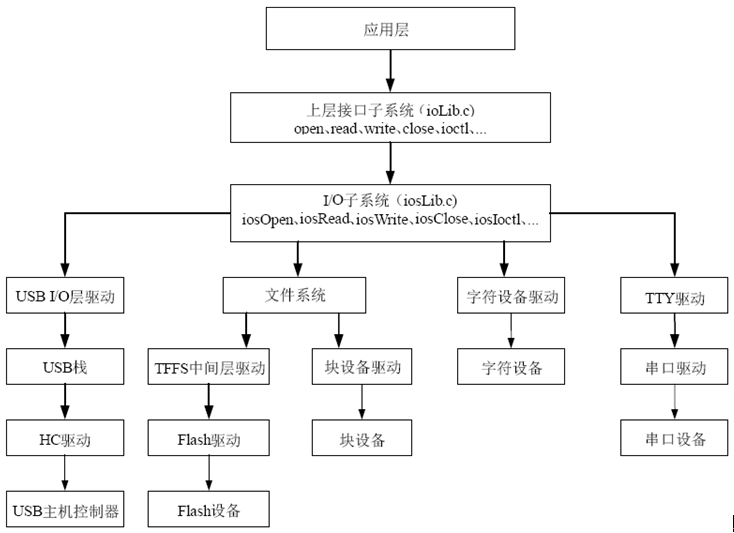
\includegraphics[width=.4\textwidth]{F:\\git\\myDocement\\毕业论文内容\\论文\\graphics\\VxWorks驱动内核层次结构.png}
\caption{VxWorks驱动内核层次结构}\label{fig:VxWorks内核驱动层次结构}
\end{figure}

	I/O 子系统在整个驱动层次中起着十分重要的作用,其对下管理着各种类型的设备驱动。换句话说,各种类型(包括网络设备)的设备都必须向I/O 子系统进行注册方可被内核访问。所以在I/O 子系统这一层次,内核维护着三个十分关键的数组用以对设备所属驱动、设备本身以及当前系统文件句柄进行管理。

	需要指出的是,VxWorks文件系统在内核驱动层次中实际上是作为块设备驱动层次中的一个中间层而存在的,其向I/O 子系统进行注册,而将底层块设备驱动置于自身的管理之下以提高数据访问的效率。在这些文件系统中,dosFs 和rawFs 是最常用的两种文件系统类型,在VxWorks早期版本就包含对这两种文件系统的支持。

\subsubsection{驱动程序管理表}
\subsubsection{驱动程序管理步骤}







\section{USB转串口设备驱动程序的实现}

\subsection{特定需求的单设备支持}


\subsection{通用的多设备支持}